% -----------------------------------------------
% Template for ISMIR LBD Papers
% 2026 version, based on previous ISMIR templates

% Requirements :
% * 2+n page length maximum
% * 10MB maximum file size
% * Copyright note must appear in the bottom left corner of first page
% * Clearer statement about citing own work in anonymized submission
% (see conference website for additional details)
% -----------------------------------------------

\documentclass{article}
\usepackage[T1]{fontenc} % add special characters (e.g., umlaute)
\usepackage[utf8]{inputenc} % set utf-8 as default input encoding
\usepackage[lbd,submission]{ismir} 
\usepackage{amsmath,cite,url}
\usepackage{graphicx}
% Figures live in figures/ in this repository; the ISMIR zip had them flat.
\graphicspath{{figures/}}
\usepackage{color}
\def\lbd{}	% Flag to use correct LBD settings in the paper, please do not modify this line


% Title. Please use IEEE-compliant title case when specifying the title here,
% as it has implications for the copyright notice
% ------
\title{Atlas Flow: Explicit Timbre-Trajectory Modeling for a Navigable Latent-Space Synthesizer}

% Note: Please do NOT use \thanks or a \footnote in any of the author markup

% Single address
% To use with only one author or several with the same address
% ---------------
%\oneauthor
% {Names}
% {Affiliations}

% Two addresses
% --------------
%\twoauthors
%  {First author} {School \\ Department}
%  {Second author} {Company \\ Address}

% Three addresses
% --------------
% \threeauthors
%   {Yuxuan Shi} {University of Pennsylvania \\ {\tt shi10@upenn.edu}}
%   {Second Author} {\bf Retain these fake authors in\\\bf submission to preserve the formatting}
%   {Third Author} {Affiliation3 \\ {\tt author3@ismir.edu}}

\multauthor
{Yuxuan Shi$^{1*}$ \hspace{0.5cm} Yifeng Huang$^{2*}$ \hspace{0.5cm} Jiangnan Zhang$^{3*}$ \hspace{0.5cm} Jinyue Guo$^{4}$ \hspace{0.5cm} Jiayi Hu$^{5\dagger}$}
{ $^1$ University of Pennsylvania, Philadelphia, USA\\
  $^2$ Fudan University, Shanghai, China\\
  $^3$ Shanghai Conservatory of Music, Shanghai, China\\
  $^4$ RITMO, University of Oslo, Oslo, Norway\\
  $^5$ TwiddleAI, Shanghai, China\\
  {\tt\footnotesize shi10@upenn.edu, yfhuang24@m.fudan.edu.cn, johngoner@icloud.com, jinyue.guo@imv.uio.no, jiayifdzl@gmail.com}\\
  $^{*}$ Equal contribution. \hspace{0.3cm} $^{\dagger}$ Corresponding author.}
  
% Four or more addresses
% OR alternative format for large number of co-authors
% ------------
%\multauthor
%{First author$^1$ \hspace{1cm} Second author$^1$ \hspace{1cm} Third author$^2$} { \bfseries{Fourth author$^3$ \hspace{1cm} Fifth author$^2$ \hspace{1cm} Sixth author$^1$}\\
%  $^1$ Department of Computer Science, University , Country\\
%$^2$ International Laboratories, City, Country\\
%$^3$  Company, Address\\
%{\tt\small CorrespondenceAuthor@ismir.edu, PossibleOtherAuthor@ismir.edu}
%}

% For the author list in the Creative Common license and PDF metadata, please enter author names. 
% Please abbreviate the first names of authors and add 'and' between the second to last and last authors.
% \def\authorname{F. Author, S. Author, and T. Author}
\def\authorname{Y. Shi, Y. Huang, J. Zhang, J. Guo, and J. Hu}
% Optional: To use hyperref, uncomment the following.
%\usepackage[bookmarks=false,pdfauthor={\authorname},pdfsubject={\papersubject},hidelinks]{hyperref}
% Mind the bookmarks=false option; bookmarks are incompatible with ismir.sty.

\sloppy % please retain sloppy command for improved formatting

\begin{document}

%
\maketitle
%
\begin{abstract}
We introduce \textit{Atlas Flow}, a real-time interactive
timbre-morphing system for MIDI-based music production. Given a fixed
MIDI sequence, it renders the sequence while exposing a two-dimensional
map of a learned 128-dimensional timbre space, obtained by principal
component analysis over training trajectories, with instrument presets
as labeled anchors. The user draws a path across this map; the path is
read as a sequence of anchor coordinates, and a conditional
flow-matching model generates the frame-rate 128-dimensional latent
trajectory around them. A causal, PQMF-based decoder in the manner of
BRAVE renders audio from that trajectory, with MIDI pitch injected as a
FiLM condition at every stage. Because each coordinate returns a trajectory
rather than a single latent vector, timbre keeps morphing through a held note,
and a path drawn across the map becomes timbre automation of the take. 
% The 22.2\,M-parameter model needs no GPU and ships as a self-contained desktop application.
\end{abstract}
%
\section{Introduction \& Related Work}\label{sec:introduction}

Learned timbre spaces are well studied: perceptually regularized latent
spaces~\cite{esling2018generativetimbrespacesregularizing}, conditioned
autoencoders that interpolate in real
time~\cite{colonel2020conditioningautoencoderlatentspaces,puche2021caesynthrealtimetimbreinterpolation},
latent timbre synthesis and its sound-design
practice~\cite{Tatar_2020,tatar2023sounddesignstrategieslatent}, and
preset-space interpolation~\cite{10596701}. Pitch is usually handled by
conditioning; CAESynth~\cite{puche2021caesynthrealtimetimbreinterpolation}
adds adversarial regularization, which we adopt.
RAVE~\cite{caillon2021ravevariationalautoencoderfast} and
DDSP~\cite{engel2020ddspdifferentiabledigitalsignal} showed that neural
synthesis can run faster than real time on commodity hardware.

These systems share two limits. First, RAVE-style latents are coarse:
each vector summarizes 2048 samples, and
BRAVE~\cite{caspe2025designingneuralsynthesizerslowlatency} shows the
resulting jitter (spanning 46.4\,ms) and loudness and pitch errors shrink
as compression decreases. Second, they encode
trajectories from existing audio; driven from a control surface, there is
none to encode. Latent Terrain~\cite{zheng_latent_2026} maps XY
coordinates directly into a RAVE latent space, but like a knob it returns
one latent vector per coordinate, so any timbral motion within a note
must be performed by hand.

We instead have each coordinate return a \emph{trajectory}. Over a fixed
MIDI sequence, the system shows a two-dimensional map of a learned timbre
space (the \emph{atlas}) with presets as labeled anchors, and renders the
sequence while its timbre follows a pointer, so a path traced across the
atlas becomes timbre automation for the take. A \emph{flow predictor}
generates these trajectories from atlas coordinates. It is trained with
conditional flow
matching~\cite{lipman2023flowmatchinggenerativemodeling}, whose
straight-line probability paths permit few-step integration and which has
recently been made streamable for
audio~\cite{liang2025binauralflowcausalstreamableapproach}. A
pitch-invariant encoder supplies its training targets, and a
MIDI-conditioned decoder renders the result.

\section{Method}

\subsection{Training}

Training runs in three phases, all using AMP fp16, gradient clipping at
$1.0$ and $1000$ warm-up updates.


\begin{figure*}[!t]
\centerline{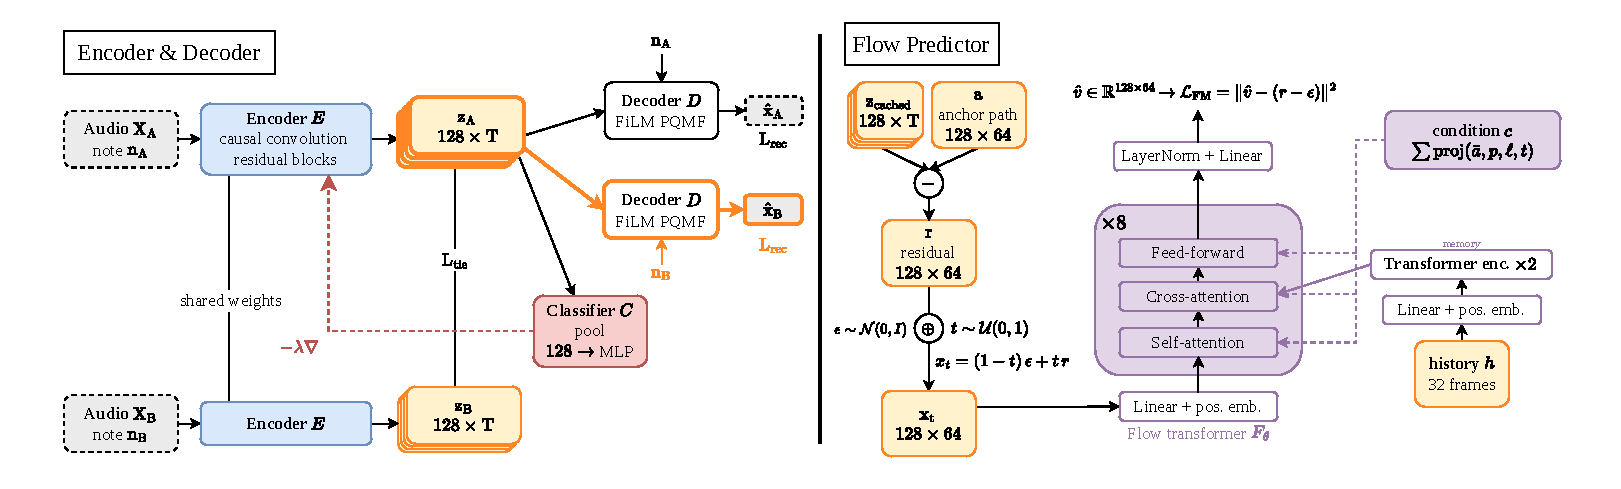
\includegraphics[width=0.85\textwidth]{atlas-flow-training.pdf}}
\caption{Training. \textbf{Left:} phase 1, encoder and decoder.
\textbf{Right:} phase 2, flow predictor.}
\label{fig:training}
\end{figure*}



\noindent\textbf{Phase 1: encoder and decoder, 60k updates.}
A shared encoder maps the paired renders $x_A$ at note $n_A$ and $x_B$
at $n_B$ to $z_A$ and $z_B$. The decoder runs twice on $z_A$,
against its own note and against the other's, giving
$\hat{x}_A = D(z_A, n_A)$ and $\hat{x}_B = D(z_A, n_B)$; each is scored
against the corresponding real render, and \emph{$z_B$ is never
decoded}. This cross branch is the heart of the design: asking A's
timbre to render B's note means any pitch stored in $z$ emerges at the
wrong pitch, where the reconstruction loss punishes it ---
multi-resolution STFT (1.0), a short-window multiband term for
transients (0.5), envelope (0.1) and RMS (0.25), averaged over both
branches. Two lighter terms escalate that demand.
$\mathcal{L}_\mathrm{tie}$ (0.1) ties $z_A$ to $z_B$, so pitch may not
\emph{vary} with the note; $\mathcal{L}_\mathrm{adv}$ (0.05) adds that
it may not be \emph{detectable}, a classifier predicting the note from
the pooled trajectory through a gradient-reversal layer, learning to
find pitch as the encoder learns to remove
it~\cite{ganin2015unsuperviseddomainadaptationbackpropagation}.

\noindent\textbf{Phase 2: flow predictor, 100k updates.}
Phase 1 yields trajectories only by encoding existing audio, phase 2 caches them as targets and learns to produce
them from a coordinate. Each preset carries an \emph{anchor} $\bar{a}$,
the median across renders of each render's temporal median; an anchor
path $a$ repeats it across a 64-frame window, or smoothsteps between two
anchors over $0.5$\,s when the gesture crosses presets. The predictor
models only the residual $r = z - a$: the atlas supplies which preset,
the network how the timbre moves within it. Windows arrive as full plans
(40\%, no real history), continuations (40\%,) from 32 genuine frames; and a \emph{preset switch} (20\%) with history and target from different presets. 
% The
% switch is the only task in which the model sees a move between presets,
% and is what makes interactive morphing possible.

The objective is conditional flow matching on that residual. With
$\epsilon \sim \mathcal{N}(0,I)$ and $t \sim \mathcal{U}(0,1)$, the
network sees $x_t = (1-t)\epsilon + t r$ and regresses the velocity
$r - \epsilon$ (1.0). Auxiliary terms tie the first generated frame to
the last history frame (0.10), match per-channel statistics (0.02) and
match first and second temporal differences (0.05). The boundary term
earns its keep at inference, where windows are concatenated with no
crossfade.

\noindent\textbf{Phase 3: joint, 30k updates.} Both objectives are summed over all modules, with a further term (0.10)
tying the live encoder output to the cached trajectories.

\subsection{Inference}\label{sec:inference}

At inference, the pointer
gives two atlas dimensions and a Gaussian-weighted blend of nearby
presets gives the other six; the point is then expressed as an
inverse-distance mixture of the nearest 128-D anchors, within the
connected component of the nearest preset, so every gesture stays a
mixture of presets the model has seen and neighbouring coordinates sound
alike. Routing from the current position to the target over the mutual
4-NN graph, traversed with a smoothstep $3t^2-2t^3$ over $0.5$\,s, gives
the anchor path $a$; its zero endpoint derivatives let a morph start and
stop without a discontinuity in rate.

The predictor integrates from noise to $\hat{r}$ with a four-step Heun
solver in autoregressive 64-frame blocks, each conditioned on the
previous 32 generated frames; the decoder then renders
$\hat{z} = a + \hat{r}$ against the MIDI note, which enters the decoder
alone.


% \section{Results}\label{sec:results}


\subsection{The trained model}\label{sec:system}

The trained model has three learned parts, 22.2\,M parameters in total.
The \textbf{encoder} (0.63\,M) is a causal convolutional stack that maps
pitch-normalized features (harmonic magnitudes sampled at multiples of
the known $f_0$, plus frame statistics) to a $\tanh$-bounded
128-dimensional trajectory at one frame per 46.4\,ms. The \textbf{flow
predictor} (13.5\,M) is a transformer with two layers encoding the
history and eight decoder layers, each modulated by adaptive LayerNorm
from a per-frame conditioning vector: anchor path, 8-D atlas path, a
lifecycle signal (age, gate, release, onset) and flow time. It never
sees MIDI, so it cannot encode pitch as timbre, and pitch accuracy rests
entirely on the decoder. The \textbf{decoder} (7.9\,M) is a causal
PQMF-based network after
BRAVE~\cite{caspe2025designingneuralsynthesizerslowlatency}. Unlike a
timbre-transfer decoder, it receives MIDI as a bounded FiLM condition at
every residual block rather than estimating pitch from audio, alongside
a parameter-free, phase-continuous harmonic excitation built from the
note frequency.

\subsection{A self-contained application}

\begin{figure}[!htb]
\centerline{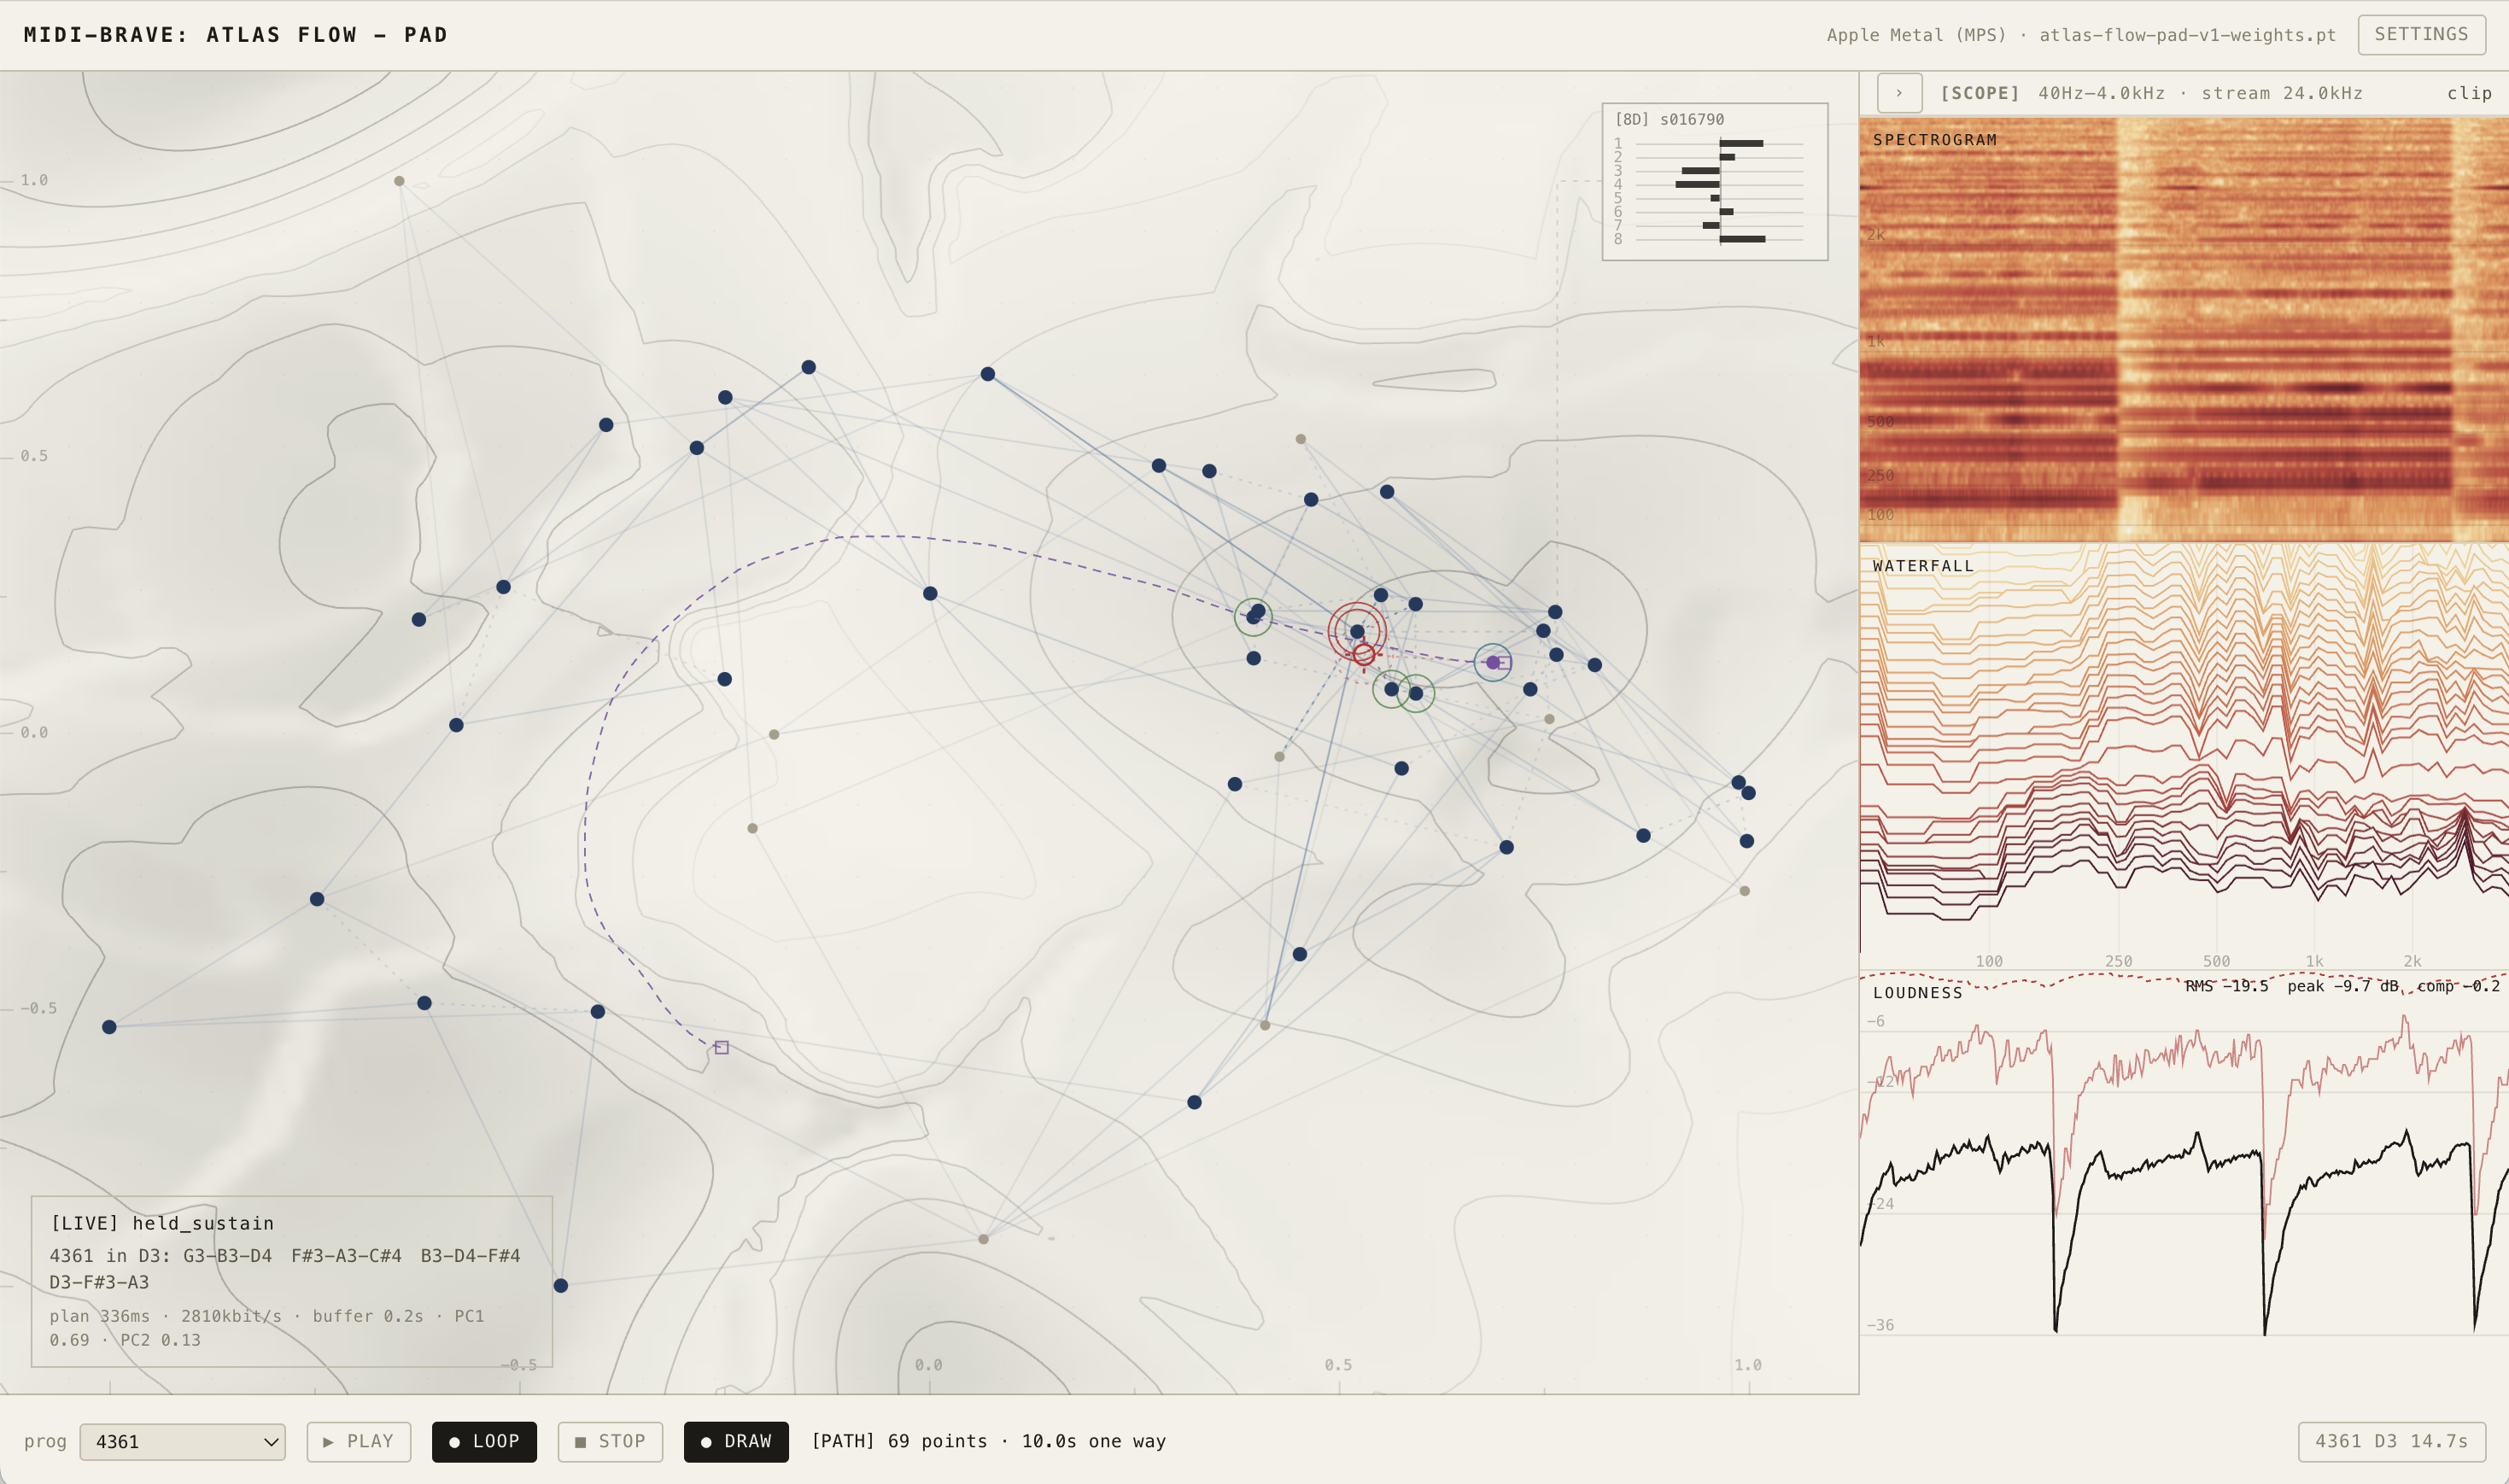
\includegraphics[width=\columnwidth]{atlas-flow-UI-paper-light.png}}
\caption{The application UI. The atlas contains preset
anchors as dots, their nearest-neighbour edges, and shading by how far a request
at each point is projected before reaching the model.}
\label{fig:atlas-flow-UI}
\end{figure}

The model ships as a self-contained desktop application for macOS and
Windows (Figure~\ref{fig:atlas-flow-UI}). It runs entirely locally and
plays smoothly on a standard CPU, with no GPU or network required. Code
and project materials are available at
\url{https://github.com/Twiddle-AI-China/MIDI-Brave}.



% \section{AI Usage Statement}

% In line with the ISMIR 2026 AI Usage Policy, if you need to declare and explain the use of AI tools in the work described in the paper, you can do so by including a section titled ``AI Usage Statement" at the end of the paper. The AI Usage Statement section can be included both at submission time and in your camera-ready version. See the Call for Late-breaking Demo and Author Guidelines for more details. The AI Usage Statement section does \textit{not} count towards the page limit for scientific content. 


% For bibtex users:
\bibliography{ISMIRtemplate}

% For non bibtex users:
%\begin{thebibliography}{citations}
% \bibitem{Author:17}
% E.~Author and B.~Authour, ``The title of the conference paper,'' in {\em Proc.
% of the Int. Society for Music Information Retrieval Conf.}, (Suzhou, China),
% pp.~111--117, 2017.
%
% \bibitem{Someone:10}
% A.~Someone, B.~Someone, and C.~Someone, ``The title of the journal paper,''
%  {\em Journal of New Music Research}, vol.~A, pp.~111--222, September 2010.
%
% \bibitem{Person:20}
% O.~Person, {\em Title of the Book}.
% \newblock Montr\'{e}al, Canada: McGill-Queen's University Press, 2021.
%
% \bibitem{Person:09}
% F.~Person and S.~Person, ``Title of a chapter this book,'' in {\em A Book
% Containing Delightful Chapters} (A.~G. Editor, ed.), pp.~58--102, Tokyo,
% Japan: The Publisher, 2009.
%
%
%\end{thebibliography}

\end{document}

